\documentclass[a4paper,11pt]{scrartcl}

\usepackage[ngerman]{babel}
% uncomment or modify according to your operating system
% \usepackage[applemac]{inputenc} % european characters can be used (Mac OS)
%\usepackage[latin1]{inputenc} 
%\usepackage{ucs} % fuer deutsche Sonderzeichen unter Linux
%\usepackage[utf8x]{inputenc} %fuer deutsche Sonderzeichen unter Linux
\usepackage[utf8]{inputenc} %fuer deutsche Sonderzeichen unter Windows
\usepackage[T1]{fontenc}
\usepackage{graphicx} 
\usepackage{fullpage}
\usepackage{latexsym}
\usepackage{amssymb}
\usepackage{amsmath}
\usepackage{ifthen}
\usepackage{listings}
\usepackage{color}
\usepackage{hyperref}
\usepackage{cite}
\usepackage{float}
\usepackage{subcaption} 

\definecolor{dkgreen}{rgb}{0,0.6,0}
\definecolor{gray}{rgb}{0.5,0.5,0.5}
\definecolor{mauve}{rgb}{0.58,0,0.82}


\lstset{ %
  language=Python,                % the language of the code
  basicstyle=\small,              % the size of the fonts that are used for the code
  numbers=left,                   % where to put the line-numbers
  numberstyle=\tiny\color{gray},  % the style that is used for the line-numbers
  stepnumber=1,                   % the step between two line-numbers. If it's 1, each line 
                                  % will be numbered
  numbersep=5pt,                  % how far the line-numbers are from the code
  backgroundcolor=\color{white},      % choose the background color. You must add \usepackage{color}
  showspaces=false,               % show spaces adding particular underscores
  showstringspaces=false,         % underline spaces within strings
  showtabs=false,                 % show tabs within strings adding particular underscores
  frame=single,                   % adds a frame around the code
  rulecolor=\color{black},        % if not set, the frame-color may be changed on line-breaks within not-black text (e.g. commens (green here))
  tabsize=2,                      % sets default tabsize to 2 spaces
  captionpos=b,                   % sets the caption-position to bottom
  breaklines=true,                % sets automatic line breaking
  breakatwhitespace=false,        % sets if automatic breaks should only happen at whitespace
  title=\lstname,                   % show the filename of files included with \lstinputlisting;
                                   % also try caption instead of title
  keywordstyle=\color{blue},          % keyword style
  commentstyle=\color{dkgreen},       % comment style
  stringstyle=\color{mauve},         % string literal style
  escapeinside={\%*}{*)},            % if you want to add LaTeX within your code
  morekeywords={end,sortrows}               % if you want to add more keywords to the set
}


% Abkuerzungen fuer haeufige Befehle wie z.B. griechische Buchstaben
\newcommand{\N}{\mathbb{N}}
\newcommand{\Z}{\mathbb{Z}}
\newcommand{\R}{\mathbb{R}}
\newcommand{\C}{\mathbb{C}}
\newcommand{\F}{\mathcal{F}}
\newcommand{\La}{\mathcal{L}}
\newcommand{\de}{\delta}
\newcommand{\e}{\varepsilon}
\newcommand{\la}{\lambda} 
\newcommand{\p}{\varphi} 
\newcommand{\al}{\alpha} 
\newcommand{\be}{\beta} 
\newcommand{\om}{\omega}
\newcommand{\Om}{\Omega}
\newcommand{\ta}{\tau}
\newcommand{\g}{\gamma}
\newcommand{\HE}{\mathbb{H}}
\newcommand{\E}{\mathbb{E}}
\newcommand{\vG}{\varGamma}
\newcommand{\s}{\sigma}

\begin{document}

\subject{LVA-Modeling and Simulation}
\title{Fake News}

\publishers{Supervisor: Max Mustermann}
\author{Marianne Musterfrau, Matricular Number - Curriculum Number\footnote{Created the results for case study 3 and wrote Chapter 2 of the documentation.}\\
Max Mustermann jun.,Matricular Number - Curriculum Number\footnote{Collected the data and wrote Chapter 3 of the documentation.}\\
Max Mustermann sen., Matricular Number - Curriculum Number\footnote{Implemented the base source code and evaluated case studies 1 and 2.}\\
Marianne Musterfrau sen., Matricular Number - Curriculum Number\footnote{Wrote introduction and discussion.}}

\maketitle

\begin{abstract}
Poorly written documentations of modelling projects are responsible for countless poor grades at Austrian universities. With this template, including the template abstract you are currently reading, we aim to reduce number of bad grades and improve the quality of scientific project documentations sustainably.
\end{abstract}

\newpage

\tableofcontents

\newpage

\section{Introduction}
\paragraph{Motivation.} 
\paragraph{Introduction to the Topic.} 
\paragraph{Reated Work.}
\paragraph{Aim.} 

\section{Model}
\subsection{Modelling}
\label{sec:modelling}

\subsection{Parametrization}

\subsection{Implementation}

\section{Simulation Results}

\newpage
\section{Task 4: Anti-Troll}
To counter the spread of misinformation by trolls, we have developed a series of countermeasures that progressively enhance the simulation's ability to regulate user interactions and reinforce credible sources. These countermeasures involve the introduction of trusted agents, a reporting and shadowbanning system, and a community note mechanism that collectively work to mitigate the influence of trolls.
\subsection{Trusted Agents}
The first mechanism in the simulation is the introduction of trusted agents, which represent credible news sources or verified profiles. These agents serve as authoritative voices in the network, always maintaining a belief value of 1, signifying their strong alignment with factual information. Additionally, trusted agents possess a higher convincing power, making them significantly more influential than ordinary agents. This enhancement ensures that factual content has a stronger presence in the belief network, counterbalancing the influence of trolls who aim to spread misinformation.
\paragraph{}Trusted Agents can be Introduced  via:
\begin{lstlisting}[
 escapeinside={//*}{*//},  % for line labeling
 caption={Introducing Trusted Agents},
 label=src:Intro_TrustedAgents]
 class Agent:
    def __init__(self, i, j, is_troll, belief, convincing_power, is_trusted):
        self.i = i  # Grid x-coordinate
        self.j = j  # Grid y-coordinate
        self.is_troll = is_troll  # Boolean indicating if the agent is a troll
        self.belief = belief  # Belief value between [-1, 1]
        self.convincing_power = convincing_power  # Influence strength [0, cmax]
        self.is_trusted = is_trusted  # Boolean indicating if the agent is trusted  //* \label{lnbr:is_trusted_def} *//

# Parameters
N = 10000  # Population size
cmax = 0.5  # Maximum convincing power
p_plus = 0.8  # Fraction of initial positive beliefs
grid_size = int(np.sqrt(N))  # Grid dimensions
timesteps = 3000  # Simulation duration
troll_frac = 0.211
trusted_frac = 0.05

# Initialize grid and agents
grid = []
for i in range(grid_size):
    row = []
    for j in range(grid_size):
        is_troll = np.random.rand() < troll_frac
        is_trusted = np.random.rand() < trusted_frac                     //* \label{lnbr:is_trusted_def} *//
        if is_troll:
            belief = -1.0
        else:
            if is_trusted:
                belief = 1.0                                             //* \label{lnbr:is_trusted_belief} *//
            else:
                belief = np.random.uniform(0, 1) if np.random.rand() < p_plus else np.random.uniform(-1, 0)
        convincing_power = (
            np.random.uniform(0, cmax) + np.random.uniform(0, 0.2)       //* \label{lnbr:is_trusted_conv} *//
            if is_trusted
            else np.random.uniform(0, cmax)
        )
        row.append(Agent(i, j, is_troll, belief, convincing_power, is_trusted))
    grid.append(row)
\end{lstlisting}   

In the initial version of the model, all agents, followed the same belief update mechanisms without distinguishing between credible sources and unverified individuals. The improved version introduces the \verb|is_trusted|(row\ref{lnbr:is_trusted_def}) attribute, which explicitly identifies trusted agents. These agents are assigned a belief value of \verb|1|(row\ref{lnbr:is_trusted_belief}), and their convincing power is increased by adding an additional random value to their base power(row\ref{lnbr:is_trusted_conv}). 

\subsection{Reporting and Shadow Banning}
While the introduction of trusted agents strengthens the credibility of information sources, it does not directly address the presence of trolls. To mitigate the impact of trolls spreading misinformation, we introduced a reporting and shadow banning system. This mechanism allows users to report trolls when they detect misinformation. When an agent accumulates a certain amount of reports, they become shadowbanned, significantly reducing their influence in the network.
\paragraph{}The implementation of agent reporting and shadow banning is achieved via:
\begin{lstlisting}[
 escapeinside={//*}{*//},  % for line labeling
 caption={Introducing Reporting and Shadow Banning},
 label=src:Intro_Reporting&ShadowBanning]
class Agent:
    def __init__(self, i, j, is_troll, belief, convincing_power, is_trusted):
        self.reports = 0  # Number of reports received
        self.shadowbanned = False  # Shadowban status

    @property
    def effective_convincing_power(self):
        """Return the convincing power, halved if the agent is shadowbanned."""
        return self.convincing_power / 2 if self.shadowbanned else self.convincing_power     

    # Parameters
    report_threshold = 5  # Reports required to shadowban a user                                 

   # Simulate user-driven protections
    interactors = random.sample(
        [agent for row in grid for agent in row if not agent.shadowbanned],
        k=int(0.1 * N)
    )

    for i in range(0, len(interactors), 2):
        if i + 1 >= len(interactors):
            break
        a1, a2 = interactors[i], interactors[i + 1]

        # Simulate content flagging
        if a1.is_troll and not a2.is_troll:
            if random.random() < 0.7:
                a1.reports += 1
        elif a2.is_troll and not a1.is_troll:
            if random.random() < 0.7:
                a2.reports += 1

    # Apply shadowban based on report threshold
    for row in grid:
        for agent in row:
            if agent.reports >= report_threshold:
                agent.shadowbanned = True
\end{lstlisting}   

Shadowbanning is implemented by adding a \verb|reports| attribute to each agent, which keeps track of the number of times they have been reported. Users report trolls with a 70\% probability, and once the threshold of five reports is reached, the agent is shadowbanned. When shadowbanned, the agent's convincing power is reduced by half, making them less effective at spreading their beliefs.This mechanism ensures that the system remains self-regulating, as users collectively reduce the impact of trolls by flagging misinformation when encountered.

\subsection{Community Notes}
While shadowbanning trolls reduces their influence, it does not actively correct misinformation that may have already spread within the network. To address this, we implemented community notes, which act as a fact-checking mechanism driven by collective disagreement among agents. If an agent believes in fake news (i.e., holds a negative belief), but the majority of its neighbors disagree, a community note is triggered. This mechanism encourages the agent to shift their belief toward the accurate information.

\begin{lstlisting}[
 escapeinside={//*}{*//},  % for line labeling
 caption={Introducing Community Notes},
 label=src:Intro_CommunityNotes]
class Agent:
# Parameters
community_note_threshold = 2  # Number of disagreements required to trigger community notes

  if agent.belief < 0:
            # Track the number of disagreements with neighbors
            disagreements = sum(
                1 for nb in neighbors if not nb.is_troll and np.sign(nb.belief) != np.sign(agent.belief)
            )

            # Apply community notes effect if disagreements exceed threshold
            if disagreements > community_note_threshold:
                agent.belief += 0.1  # Increase belief in true news
\end{lstlisting}  

With the introduction of community notes, an additional rule is introduced: If an agent's belief contradicts its neighbors, the system actively nudges their belief toward positive values. This change ensures that misinformation is corrected over time, making it harder for false narratives to persist in the network.

In the final enhancement, we made the community notes system more aggressive against trolls. While in previous implementations, community notes only affected non-troll agents, in the latest iteration, trolls now lose an additional 30\% of their convincing power whenever they are flagged by a community note. This ensures that trolls gradually lose their ability to influence others, further weakening their role in the simulation.

\begin{lstlisting}[
 escapeinside={//*}{*//},  % for line labeling
 caption={Enhancement of Community Notes},
 label=src:Intro_CommunityNotes+]
class Agent:
         # Apply community notes effect:
            if disagreements > community_note_threshold:
                # For non-troll agents with belief < 0, increase belief
                if not agent.is_troll:
                    agent.belief += 0.1  # Increase belief, clip to [-1, 1] later
                    agent.belief = np.clip(agent.belief, -1, 1)  # Ensure belief remains within bounds

                # For troll agents, decrease convincing power
                else:
                    agent.convincing_power *= 0.7  # Reduce convincing power by 30%
\end{lstlisting}  

The new implementation modifies the community note mechanism by adding a condition that directly reduces a troll’s convincing power if they are repeatedly contradicted by their neighbors.This final step ensures that trolls become less effective over time, reinforcing an adaptive and self-correcting information ecosystem.

\subsection{Simulation Results}

\begin{figure}[!h]
    \centering
    \begin{subfigure}[b]{0.45\textwidth}
        \centering
        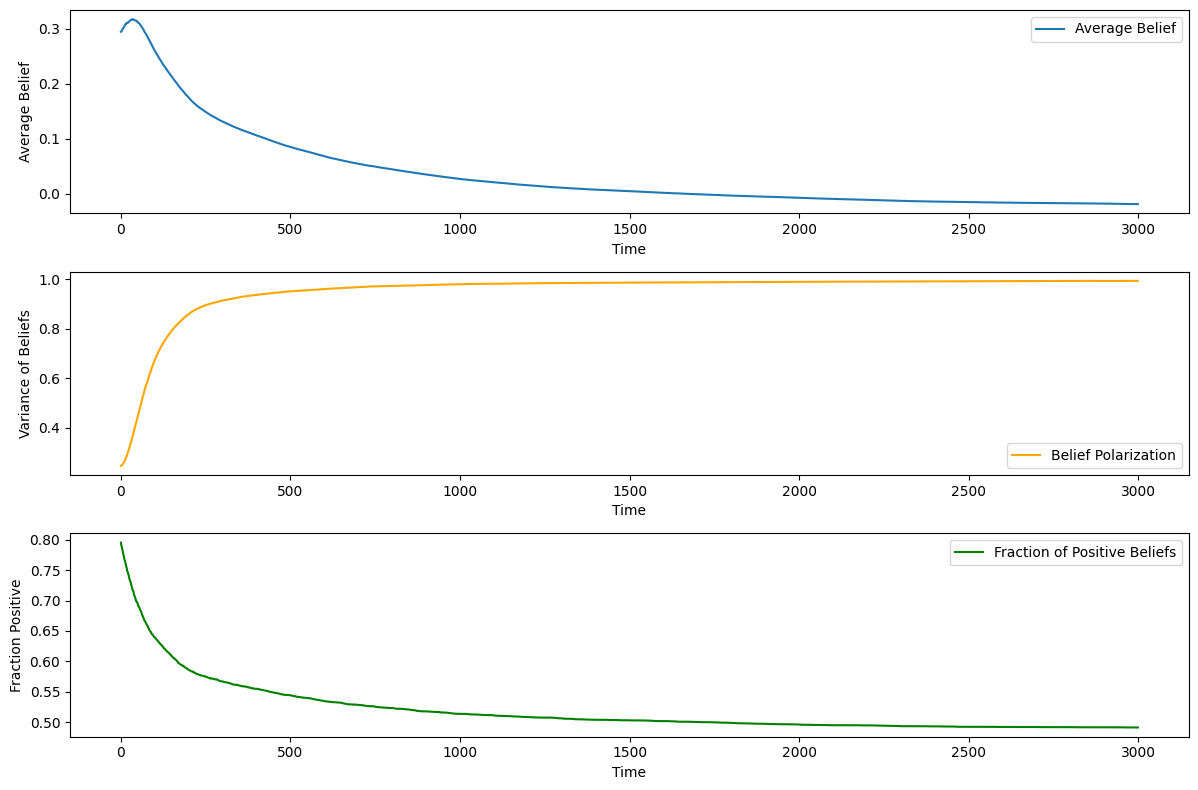
\includegraphics[width=\textwidth]{./images/task4_1.png}
        \caption{Baseline Case: No Interventions}
        \label{fig:task4_1}
    \end{subfigure}
    
    \vspace{0.5cm} 

    \begin{subfigure}[b]{0.45\textwidth}
        \centering
        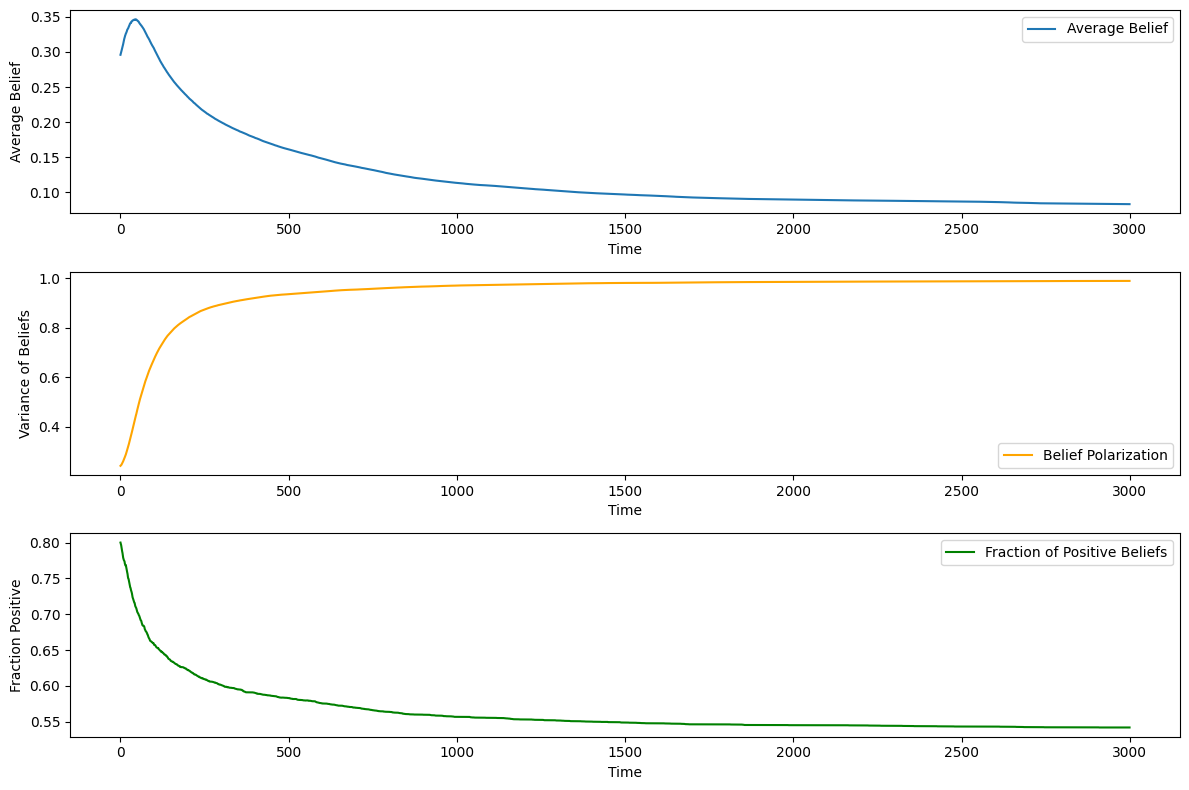
\includegraphics[width=\textwidth]{./images/task4_2.png}
        \caption{Impact of Trusted Agents}
        \label{fig:task4_2}
    \end{subfigure}
     \hfill 
    \begin{subfigure}[b]{0.45\textwidth}
        \centering
        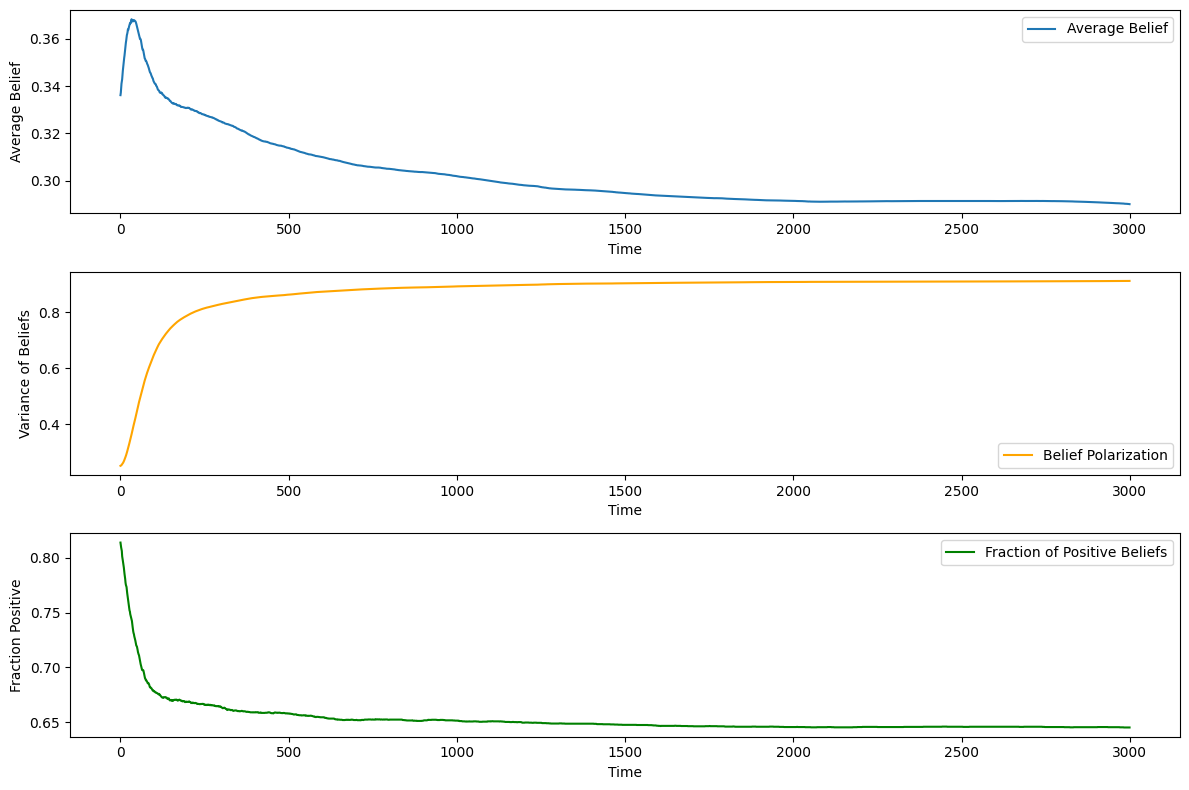
\includegraphics[width=\textwidth]{./images/task4_3.png}
        \caption{Effect of Reporting and Shadow Banning}
        \label{fig:task4_3}
    \end{subfigure}
    
    \vspace{0.5cm}

    \begin{subfigure}[b]{0.45\textwidth}
        \centering
        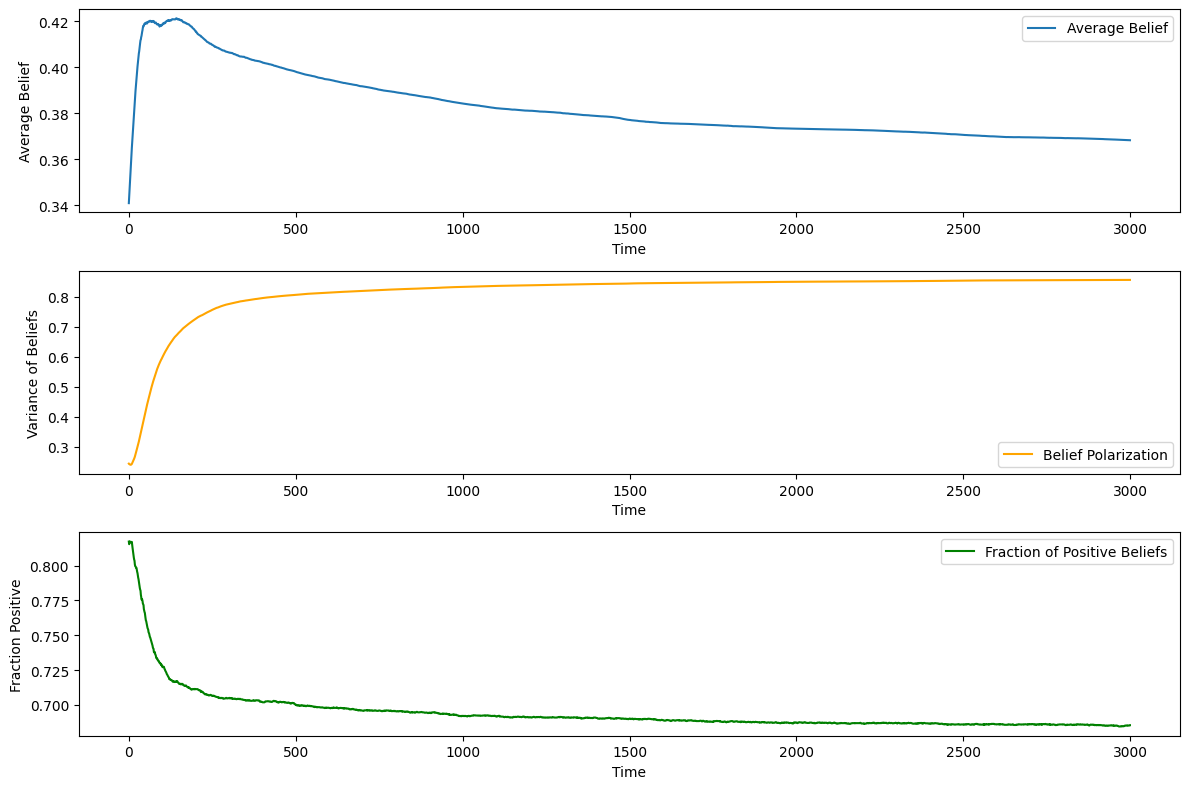
\includegraphics[width=\textwidth]{./images/task4_4.png}
        \caption{Community Notes for Belief Correction}
        \label{fig:task4_4}
    \end{subfigure}
    \hfill
    \begin{subfigure}[b]{0.45\textwidth}
        \centering
        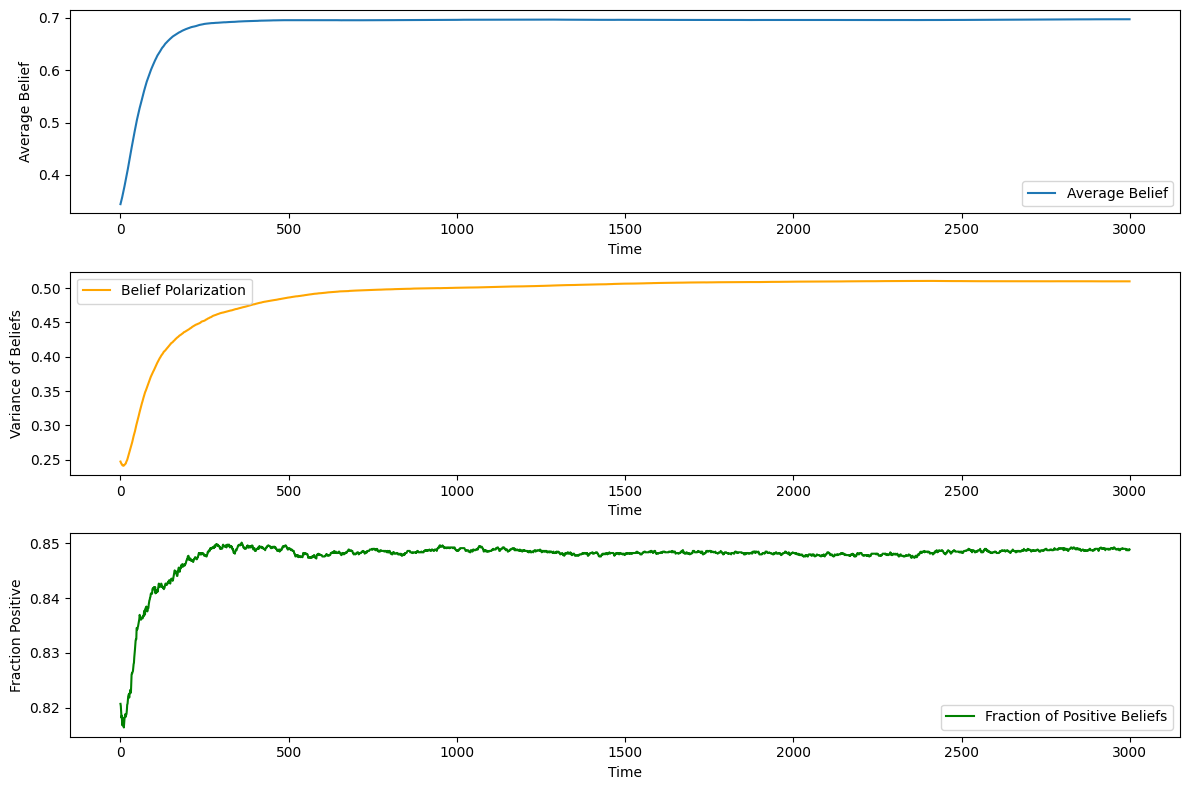
\includegraphics[width=\textwidth]{./images/task4_5.png}
        \caption{Troll Influence Reduction via Community Notes}
        \label{fig:task4_5}
    \end{subfigure}

    \caption{Simulation Results:Task 4}
    \label{fig:task4_Results}
\end{figure}

The simulation results demonstrate the progressive impact of different countermeasures against misinformation. In the baseline model (see in Figure \ref{fig:task4_1}), misinformation spreads freely, leading to a steady decline in average belief, high polarization, and a decreasing fraction of positive beliefs. Introducing trusted agents (see in Figure \ref{fig:task4_2}) slows misinformation spread but does not prevent polarization. The reporting and shadow banning mechanism (see in Figure \ref{fig:task4_3}) further stabilizes belief dynamics by reducing the influence of trolls, lowering polarization, and slowing the decline of accurate beliefs. The implementation of community notes (see in Figure \ref{fig:task4_4}) provides an effective correction mechanism, stabilizing the average belief and preventing further misinformation propagation. The final iteration, reducing troll influence after community notes (see in Figure \ref{fig:task4_5}), achieves the best results, significantly increasing average belief, reducing polarization, and maximizing the fraction of positive beliefs. These findings highlight that a combination of trusted sources, user-driven moderation, and community fact-checking is essential for mitigating misinformation and maintaining belief stability.

\newpage
\section{Discussion}
\paragraph{Summary.}
\paragraph{Result Interpretation}
\paragraph{Conclusion.} 
\paragraph{Outlook.} 
\newpage

\bibliographystyle{plain}
\bibliography{references}

\appendix
\section{Appendix}
\subsection{Not Quite Relevant Enough}
Some stuff which is not quite important enough for the main text.
\end{document}